\documentclass[a4paper,14pt]{extreport}
\usepackage[left=1.5cm,right=1.5cm,
    top=1.5cm,bottom=1.5cm,bindingoffset=0cm]{geometry}
\usepackage{scrextend}
\usepackage[T1,T2A]{fontenc}
\usepackage[utf8]{inputenc}
\usepackage[english,russian,ukrainian]{babel}
\usepackage{tabularx}
\usepackage{amssymb}
\usepackage{color}
\usepackage{amsmath}
\usepackage{mathrsfs}
\usepackage{listings}
\usepackage{graphicx}
\graphicspath{ {./images/} }
\usepackage{lipsum}
\usepackage{xcolor}
\usepackage{hyperref}
\usepackage{tcolorbox}
\usepackage{tikz}
\usepackage[framemethod=TikZ]{mdframed}
\usepackage{wrapfig,boxedminipage,lipsum}
\mdfdefinestyle{MyFrame}{%
linecolor=blue,outerlinewidth=2pt,roundcorner=20pt,innertopmargin=\baselineskip,innerbottommargin=\baselineskip,innerrightmargin=20pt,innerleftmargin=20pt,backgroundcolor=gray!50!white}
 \usepackage{csvsimple}
 \usepackage{supertabular}
\usepackage{pdflscape}
\usepackage{fancyvrb}
%\usepackage{comment}
\definecolor{ggreen}{rgb}{0.4,1,0}
\definecolor{amber}{rgb}{1.0, 0.75, 0.0}
\definecolor{babyblue}{rgb}{0.54, 0.81, 0.94}
\definecolor{arylideyellow}{rgb}{0.91, 0.84, 0.42}
\usepackage{array,tabularx}
\usepackage{colortbl}

\usepackage{varwidth}
\tcbuselibrary{skins}
\usepackage{fancybox}

\usetikzlibrary{calc}
\makeatletter
\newlength{\mylength}
\xdef\CircleFactor{1.1}
\setlength\mylength{\dimexpr\f@size pt}
\newsavebox{\mybox}
\newcommand*\circled[2][draw=blue]{\savebox\mybox{\vbox{\vphantom{WL1/}#1}}\setlength\mylength{\dimexpr\CircleFactor\dimexpr\ht\mybox+\dp\mybox\relax\relax}\tikzset{mystyle/.style={circle,#1,minimum height={\mylength}}}
\tikz[baseline=(char.base)]
\node[mystyle] (char) {#2};}
\makeatother

\usepackage{float}
\usepackage{wrapfig}
\usepackage{framed}


\begin{document}
\pagecolor{white}


\begin{center}
Variant №4\\
\vspace{0.5cm}
Bohdan Lyshchenko DP-82
\end{center}

\begin{center}
Яка модель і рівняння описують дисперсію $\varepsilon*(\omega)$ для іонної поляризації?
\end{center}
\vspace{1cm}





Ion crystals are a large and important class of dielectrics. In addition to the displacement of the electron shells of ions, the main mechanism of polarization of such crystals are electrically induced elastic displacements of ions - charged in the crystal lattice of charged particles.

Assuming that the oscillator $ m \dfrac {d^2} {dt^2} = -cx $ characterizes elastic ion polarization (lower frequency compared to
 electronic), then in the equation \ ref {q2} (The formula explains the frequency of the dielectric constant at resonant dispersion). $ \delta
  \varepsilon = \varepsilon_{\text{іч}} $, because ionic polarization is dispersed in the infrared (IR) frequency range, and in addition, the value of $ \varepsilon (\omega) $ contains a contribution from more
   high-frequency electronic polarization (optical contribution):

\begin{align}
  \varepsilon(\omega)=\varepsilon_{\mathrm{om}}+\frac{N q^{2} /\left(\varepsilon_{0} m \omega_{T O}^{2}\right)}{1-\left(\omega / \omega_{T O}\right)^{2}}
\label{q1}
\end{align}

\begin{align}
\varepsilon(\omega)=1+\frac{\Delta \varepsilon}{1-\left(\frac{\omega}{\omega_{0}}\right)^{2}} ; \quad \Delta \varepsilon=\frac{N q^{2}}{\varepsilon_{0} m \omega_{0}^{2}}
\label{q2}
\end{align}

The frequency of the oscillator $ \omega_{TO} $ corresponds to one of the natural frequencies of the ionic crystal lattice.

Ionic (infrared) mechanism of elastic polarization and determines primarily the dielectric constant of ionic crystals. Therefore, this mechanism should be considered in more detail, clarifying the physical understanding of the resonant frequency of the FTO oscillator. As with electron polarization, below this frequency

The ionic (infrared) mechanism of elastic polarization i determines primarily the dielectric constant of ionic crystals. Therefore, this mechanism should be considered in more detail, clarifying the physical understanding of the resonant frequency of the FTO oscillator. As with electron polarization, below this frequency $ \left (\omega <\omega_{T O} \right) $ static dielectric constant

Above the frequency, the Fto ion polarization is delayed (there is a dispersion of the dielectric constant in the range $ 10^{12} \ldots 10^{14} $ Hz), and therefore only optical (electronic) polarization remains at a higher frequency.

Elastic polarization in ionic crystals, which determines the resonant dependence of the dielectric constant on frequency, is described by a dynamic model of the crystal lattice. Next, we consider simple models of a one-dimensional crystal, first a linear chain of atoms that is in equilibrium under the action of forces of attraction and repulsion (Fig. $ 1, a $). The potential relief of each of the atoms is characterized by a parabolic potential well, and the oscillations of the atoms are characterized by a model of a harmonic oscillator. Suppose first that the masses of atoms or molecules are one-dimensional
molecular crystal). For simplicity, elastic displacements are considered
possible only along the chain; in addition, interactions only between the nearest neighboring atoms are taken into account.

\begin{figure}[h]
\center{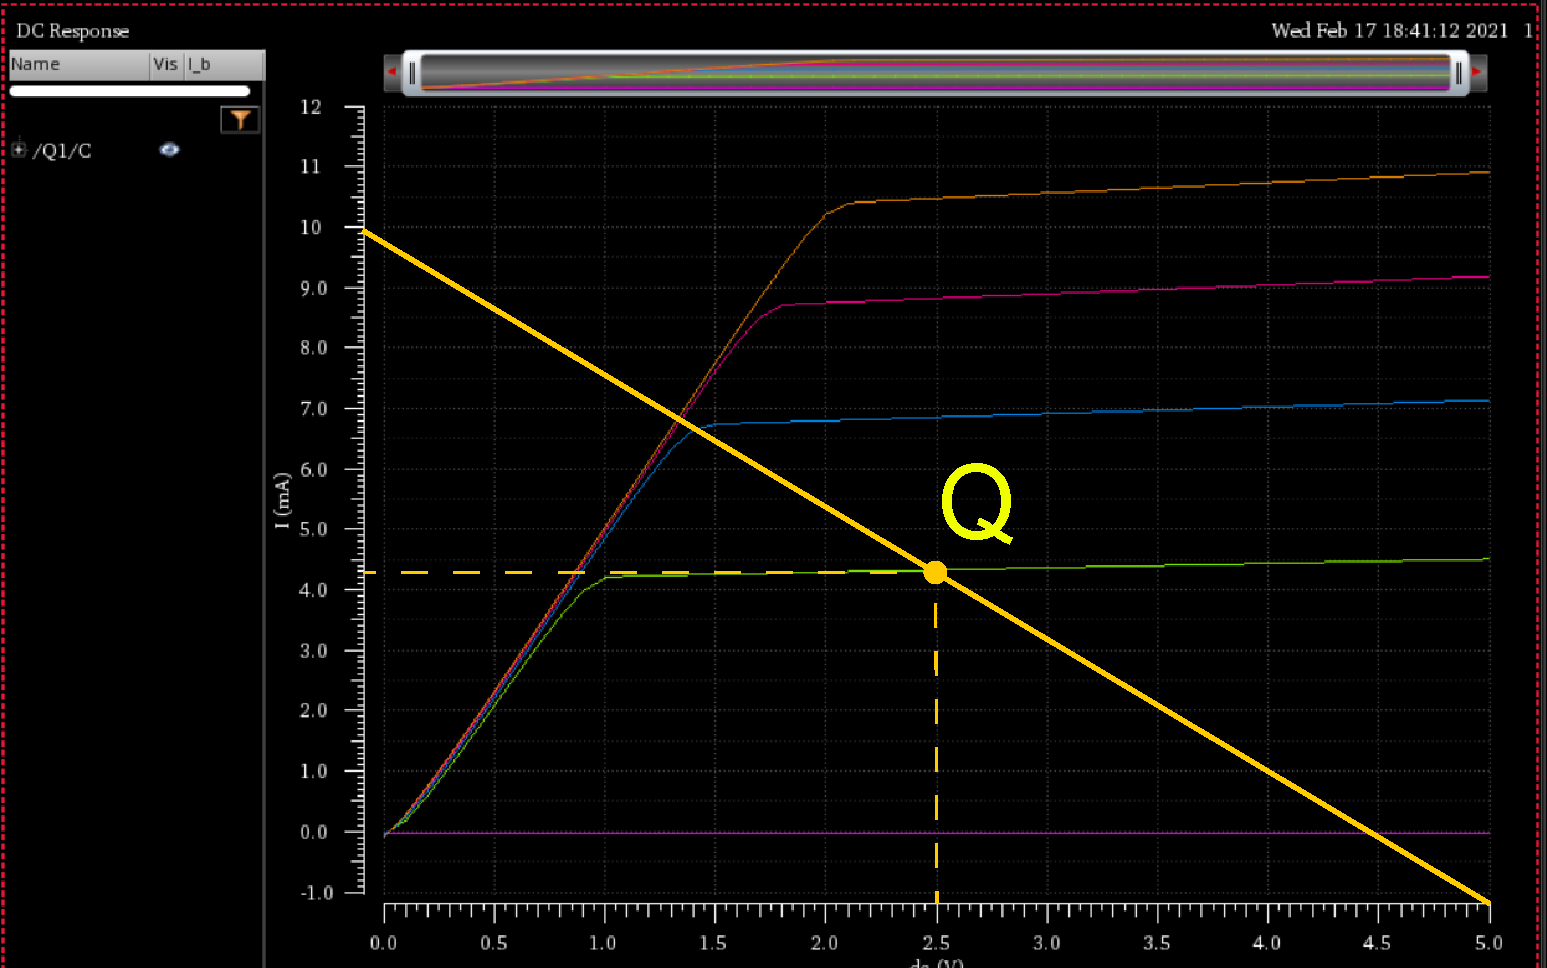
\includegraphics[width=0.7\linewidth]{1.png}}
\caption{Oscillator model and electromagnetic wave dispersion:
a - the simplest oscillator; b - resonant dispersion of the oscillator system;
in - dispersion of electromagnetic waves in vacuum and dielectric.}
\label{ris1}
\end{figure}







\end{document}
